%%%%%%%%%%%%%%%%%%%%%%%%%%%%%%%%%%%%%%%%%%%%%%%%%%%%%%%%%%%%%%%%%%%%%%%%%%%%%%%%%%%%%%%%%%%%%%%%%%%
%%%%%%%%%%%%%%%%%%%%%%%%%%%%%%%%%%%%%%%%%%%%%%%%%%%%%%%%%%%%%%%%%%%%%%%%%%%%%%%%%%%%%%%%%%%%%%%%%%%
%%%%%%%%%%%%%%%%%%%%%%%%%%%%%%%%%%%%%%%%%%%%%%%%%%%%%%%%%%%%%%%%%%%%%%%%%%%%%%%%%%%%%%%%%%%%%%%%%%%
%%%%%%%%%%%%%%%%%%%%%%%%%%%%%%%%%%%%%%%%%%%%%%%%%%%%%%%%%%%%%%%%%%%%%%%%%%%%%%%%%%%%%%%%%%%%%%%%%%%

\chapter{Espectro evolutivo}

%%%%%%%%%%%%%%%%%%%%%%%%%%%%%%%%%%%%%%%%%%%%%%%%%%%%%%%%%%%%%%%%%%%%%%%%%%%%%%%%%%%%%%%%%%%%%%%%%%%

\section{Espectro evolutivo}

\begin{proposicion}
Sean $u$ y $v$ dos funciones tipo \textit{pseudo $\delta$ de Dirac}, es decir, unimodales con un
máximo  y (...). Si $u$ tiene una concentración muy alta, con relación a $v$, entonces
\begin{equation*}
\intR u(x) v(x+k) dx \approx v(k) \intR u(x) dx
\end{equation*}
\label{pseudo_d}
\end{proposicion}

%%%%%%%%%%%%%%%%%%%%%%%%%%%%%%%%%%%%%%%%%%%%%%%%%%%%%%%%%%%%%%%%%%%%%%%%%%%%%%%%%%%%%%%%%%%%%%%%%%%
%%%%%%%%%%%%%%%%%%%%%%%%%%%%%%%%%%%%%%%%%%%%%%%%%%%%%%%%%%%%%%%%%%%%%%%%%%%%%%%%%%%%%%%%%%%%%%%%%%%
%%%%%%%%%%%%%%%%%%%%%%%%%%%%%%%%%%%%%%%%%%%%%%%%%%%%%%%%%%%%%%%%%%%%%%%%%%%%%%%%%%%%%%%%%%%%%%%%%%%

%\begin{SidewaysTable}
%\centering
%\bordes{1.5}
%\begin{tabular}{c}
%\textbf{Ventanas de retrasos tipo escalamiento (1)}
%\vspace{1em}
%\end{tabular}
%
%{
%\begin{tabular}{lll}
%\toprule
%& $k(u)$ para $\abso{u} \leq 1$ & \\
%\midrule
%Bartlett &
%$\displaystyle 
%1 
%$
%& 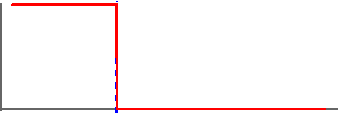
\includegraphics[scale=.66]{./img_ventanas/ventana_bartlett.pdf}
%\\
%\rowcolor{gris}
%Fejer &
%$\displaystyle 
%1-\abso{u}
%$
%& 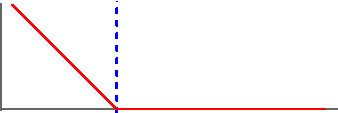
\includegraphics[scale=.66]{./img_ventanas/ventana_fejer.pdf}
%\\
%Daniell &
%$\displaystyle 
%\frac{\SEN{\pi u}}{\pi u}
%$
%& 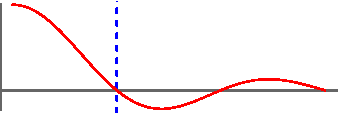
\includegraphics[scale=.66]{./img_ventanas/ventana_daniell.pdf}
%\\
%\rowcolor{gris}
%Parzen (1) &
%$\displaystyle 
%1-u^{2}
%$
%& 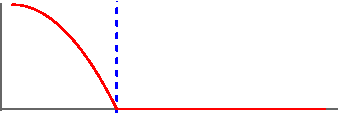
\includegraphics[scale=.66]{./img_ventanas/ventana_parzen1.pdf}
%\\
%Parzen (2) &
%$\displaystyle 
%\frac{1}{1+\abso{u}}
%$
%& 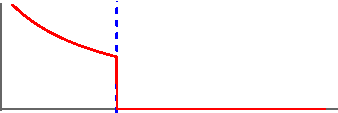
\includegraphics[scale=.66]{./img_ventanas/ventana_parzen2.pdf}
%\\
%\rowcolor{gris}
%Parzen (3) &
%$\displaystyle 
%\frac{1}{1+u^{2}}
%$
%& 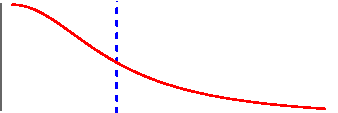
\includegraphics[scale=.66]{./img_ventanas/ventana_parzen3.pdf}
%\\
%Parzen (4) &
%$\displaystyle 
%\begin{cases}
%1-6 u^{2} + 6 \abso{u}^{3} &, \text{ si} \abso{u}\leq \nicefrac{1}{2}\\
%2\left( 1-\abso{u} \right)^{3} &, \text{ otro caso}
%\end{cases}
%$
%& 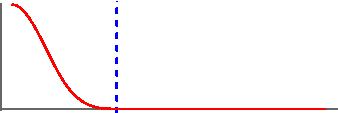
\includegraphics[scale=.66]{./img_ventanas/ventana_parzen4.pdf}
%\\
%\rowcolor{gris}
%Tukey &
%$\displaystyle 
%1 -2a +2a \COS{\pi u}
%$
%& 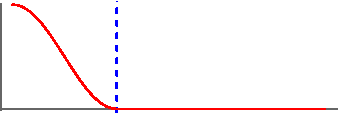
\includegraphics[scale=.66]{./img_ventanas/ventana_tukey.pdf}
%\\
%\bottomrulec
%\end{tabular}
%}
%\caption{Ejemplos de algunas ventanas que suavizan el periodograma}
%\label{ventanas}
%\end{SidewaysTable}

%%%%%%%%%%%%%%%%%%%%%%%%%%%%%%%%%%%%%%%%%%%%%%%%%%%%%%%%%%%%%%%%%%%%%%%%%%%%%%%%%%%%%%%%%%%%%%%%%%%

%\begin{SidewaysTable}
%\centering
%\bordes{1.5}
%\begin{tabular}{c}
%\textbf{Ventanas de retraso tipo escalamiento (2)}
%\vspace{1em}
%\end{tabular}
%
%{
%\begin{tabular}{lll}
%\toprule
%& $k(u)$ para $\abso{u} \leq 1$  & \\
%\midrule
%Neave &
%$\displaystyle 
%\begin{cases}
%1 &, \abso{u}\leq a \\
%\frac{1}{1-a}\left[ 1-u +\frac{b-a}{\pi}\SEN{\frac{b-u}{b-a}\pi} \right] &, a \leq \abso{u}\leq a \\
%\frac{1}{1-a}\left[ 1-u -\frac{1-b}{\pi}\SEN{\frac{u-b}{1-b}\pi} \right] &, b \leq \abso{u} \\
%\end{cases}
%$
%& 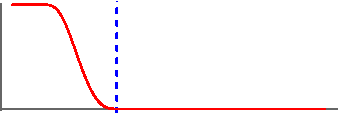
\includegraphics[scale=.66]{./img_ventanas/ventana_neave.pdf}
%\\
%\rowcolor{gris}
%Cuadrática &
%$\displaystyle 
%\frac{25}{12(\pi u)^{2}} 
%\left[ \frac{\SEN{\nicefrac{6 \pi u}{5}}}{\nicefrac{6\pi u}{5}} - \COS{\nicefrac{6 \pi u}{5}} \right]
%$
%& 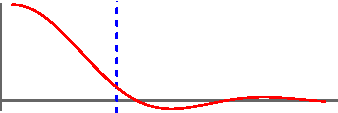
\includegraphics[scale=.66]{./img_ventanas/ventana_cuadratica.pdf}
%\\
%Bartlett-Priestley &
%$\displaystyle 
%\frac{3}{(\pi u)^{2}} \left[ \frac{\SEN{\pi u}}{\pi u} - \COS{\pi u} \right]
%$
%& 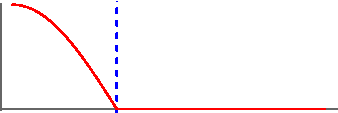
\includegraphics[scale=.66]{./img_ventanas/ventana_cosenoidal.pdf}
%\\
%\rowcolor{gris}
%Papoulis &
%$\displaystyle 
%(1-u)\COS{\pi u} + \frac{\SEN{\pi u }}{\pi u }
%$
%& 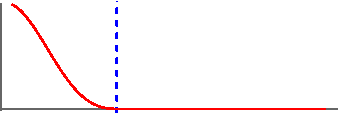
\includegraphics[scale=.66]{./img_ventanas/ventana_papoulis.pdf}
%\\
%Cosenoidal &
%$\displaystyle 
%\COS{\pi u}
%$
%\\
%\rowcolor{gris}
%Trapezoidal &
%$\displaystyle 
%\begin{cases}
%1 &, \abso{u}\leq a \\
%\frac{u-1}{a-1} &, a \leq \abso{u}\leq a 
%\end{cases}
%$
%& 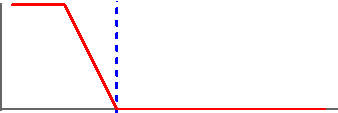
\includegraphics[scale=.66]{./img_ventanas/ventana_trapezoidal.pdf}
%\\
%Normal &
%$\displaystyle 
%\exp \left( - \nicefrac{u^{2}}{2 \sigma^{2}}  \right)
%$
%%& 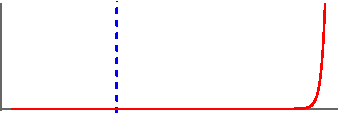
\includegraphics[scale=.66]{./img_ventanas/ventana_normal.pdf}
%& 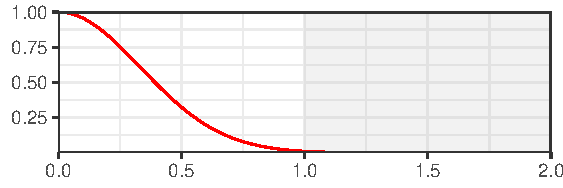
\includegraphics[scale=.66]{./img_ventanas/ventana_.pdf}
%\\
%\bottomrule
%\end{tabular}
%}
%\caption{Ejemplos de algunas ventanas que suavizan el periodograma}
%\end{SidewaysTable}

%%%%%%%%%%%%%%%%%%%%%%%%%%%%%%%%%%%%%%%%%%%%%%%%%%%%%%%%%%%%%%%%%%%%%%%%%%%%%%%%%%%%%%%%%%%%%%%%%%%
%%%%%%%%%%%%%%%%%%%%%%%%%%%%%%%%%%%%%%%%%%%%%%%%%%%%%%%%%%%%%%%%%%%%%%%%%%%%%%%%%%%%%%%%%%%%%%%%%%%
%%%%%%%%%%%%%%%%%%%%%%%%%%%%%%%%%%%%%%%%%%%%%%%%%%%%%%%%%%%%%%%%%%%%%%%%%%%%%%%%%%%%%%%%%%%%%%%%%%%

%\begin{SidewaysTable}
%\centering
%\bordes{1.5}
%\begin{tabular}{c}
%\textbf{Ventanas espectrales tipo escalamiento (1)}
%\vspace{1em}
%\end{tabular}
%
%{
%\begin{tabular}{ll}
%\toprule
%& $K(\theta)$ para $\abso{\theta} \leq 1$ \\
%\midrule
%Bartlett &
%$\displaystyle 
%\frac{1}{\pi} \frac{\SEN{\theta}}{\theta}
%$
%\\
%\rowcolor{gris}
%Fejer &
%$\displaystyle 
%\frac{1}{2\pi} \left[ \frac{\SEN{\nicefrac{\theta}{2}}}{\nicefrac{\theta}{2}} \right]^{2}
%$
%\\
%Daniell &
%$
%\displaystyle 
%\nicefrac{1}{2\pi} \text{, si } \abso{\theta}\leq \pi
%$
%\\
%\rowcolor{gris}
%Parzen (1) &
%$\displaystyle 
%d
%$
%\\
%Parzen (2) &
%$\displaystyle 
%d
%$
%\\
%\rowcolor{gris}
%Parzen (3) &
%$\displaystyle 
%d
%$
%\\
%Parzen (4) &
%$\displaystyle 
%\frac{3}{8 \pi} \left[ \frac{\SEN{\nicefrac{\theta}{4}}}{\nicefrac{\theta}{4}} \right]
%$
%\\
%\rowcolor{gris}
%Tukey &
%$\displaystyle 
%d
%$
%\\
%\bottomrulec
%\end{tabular}
%}
%\caption{Ejemplos de algunas ventanas que suavizan el periodograma}
%\end{SidewaysTable}

%%%%%%%%%%%%%%%%%%%%%%%%%%%%%%%%%%%%%%%%%%%%%%%%%%%%%%%%%%%%%%%%%%%%%%%%%%%%%%%%%%%%%%%%%%%%%%%%%%%

%\begin{SidewaysTable}
%\centering
%\bordes{1.5}
%\begin{tabular}{c}
%\textbf{Ventanas de retraso tipo escalamiento (2)}
%\vspace{1em}
%\end{tabular}
%
%{
%\begin{tabular}{ll}
%\toprule
%& $K(\theta)$ para $\abso{\theta} \leq 1$ \\
%\midrule
%Neave &
%$
%d
%$
%\\
%\rowcolor{gris}
%Cuadrática &
%$\displaystyle 
%d
%$
%\\
%Bartlett-Priestley &
%$\displaystyle 
%\frac{3}{4 \pi} \left[ 1 - \left( \nicefrac{\theta}{\pi} \right) \right]
%\text{, si } \abso{\theta}\leq \pi
%$
%\\
%\rowcolor{gris}
%Papoulis &
%$\displaystyle 
%d
%$
%\\
%Coseno &
%$\displaystyle 
%d
%$
%\\
%\rowcolor{gris}
%Trapezoidal &
%$\displaystyle 
%d
%$
%\\
%Normal &
%$\displaystyle 
%d
%$
%\\
%\bottomrule
%\end{tabular}
%}
%\caption{Ejemplos de algunas ventanas que suavizan el periodograma}
%%\label{ventanas}
%\end{SidewaysTable}

%%%%%%%%%%%%%%%%%%%%%%%%%%%%%%%%%%%%%%%%%%%%%%%%%%%%%%%%%%%%%%%%%%%%%%%%%%%%%%%%%%%%%%%%%%%%%%%%%%%

\section{Estimación del espectro evolutivo}

Una vez definido el espectro evolutivo para procesos no-estacionarios con varianza finita, cabe 
preguntarse sobre le estimación de esta cantidad a partir de una realización del proceso usando, 
por ejemplo, periodogramas modificados; tal pregunta no tiene, en general, una respuesta 
satisfactoria.
Es por ello que se define una colección, más restringida, de procesos no-estacionarios cuyo 
espectro evolutivo pueda ser estimado efectivamente usando la técnica de ventanas.

Considerando un proceso no-estacionario \xt que admite una representación de la forma 
$X(t) = \intR A(t,\omega) e^{i \omega t} dZ(\omega)$, entonces el espectro evolutivo queda definido 
como
\begin{equation}
dF_t(\omega) = \abso{A(t,\omega)}^{2} d\mu(\omega)
\label{esp_evolutivo}
\end{equation}

Antes de poder usar la proposición \ref{pseudo_d} para estimar $F_t$ (con respecto a $t$) usando 
una ventana espectral, hay que medir la dispersión de $F_t$ en el tiempo; más aún, hay que pedir 
que esa dispersión sea finita.
Con vista a la ecuación \ref{esp_evolutivo}, se puede usar la conexión entre $F$ y $A$ para 
establecer condiciones respecto a la segunda; se define entonces a $H_\omega$, la transformada de
Fourier de $A$ en el tiempo
\begin{equation}
A(t,\omega) = \intR e^{i t \theta} dH_\omega(\theta)
\end{equation}

Un motivo muy fuerte para definir un objeto tan rebuscado es que (...)

Posteriormente se define a $B_{\mathbf{F}}$, el ancho de banda para $H_\omega$ con respecto a la 
familia de funciones $\mathbf{F}$, como
%
\begin{equation}
B_{\mathbf{F}}(\omega) = \intR \abso{\theta} \abso{dH_\omega(\theta)}
\end{equation}

Se dice que el proceso es semi-estacionario con respecto a $\mathbf{F}$ si 
$\sup_\omega B_{\mathbf{F}} < \infty$. El proceso se dice simplemente \textbf{semi-estacionario} 
si esta cantidad es acotada para cualquier familia de funciones admisibles 
$\mathbf{F} \in \mathbf{C}$; entonces se puede definir la constante $B_X$, el \textit{ancho de 
banda característico de} \xt, como

\begin{equation}
B_X = \sup_{\mathbf{F}\in \mathbf{C}} \left[ \sup_\omega B_{\mathbf{F}}(\omega) \right]^{-1}
\end{equation}

Muy vagamente, $B_X$ indica el tiempo máximo en el cual el proceso, representado en la forma
\ref{esp_evolutivo}, (...)

Una vez definida la cantidad $B_X$, y habiendo supuesto que no es 0, es demostrado en 
\cite{Priestley65} que el estimador $U$ definido como en ... satisface que
%
\begin{equation}
\E{\abso{U(t,\omega)}^{2}} = \intR \abso{\Gamma(\omega)}^{2} f(t,\omega+\omega_0) d\omega
+ \orden\left( \nicefrac{B_g}{B_X} \right)
\end{equation}

De esta última expresión es evidente que el estimador es mejor conforme 
\begin{itemize}
\item  $B_X$, el tiempo máximo para el cual el proceso es \textit{básicamente estacionario}, es 
mayor
\item $B_g$, la dispersión en el tiempo para la ventana $g$, es menor
\end{itemize}

---

Entonces se ha probado en \cite{Priestley66,Priestley69} que bajo ciertas
condiciones p

\section{Estimador de doble ventana}

Respecto a la estimación del espectro local se usa el \textbf{estimador de doble ventana}, 
técnica introducida por Priestley \cite{Priestley69} y que requiere dos funciones, $w_\tau$ y 
$g$, que funcionan como ventana de retrasos y como filtro lineal, respectivamente.
%
En cuando a $g$, se define a $\Gamma(u) = \intR g(u) e^{i u \omega} du$ y se les pide que
\begin{equation*}
2\pi \int_{-\infty}^{\infty} \lvert g(u) \lvert^{2} du 
= 
\int_{-\infty}^{\infty} \lvert \Gamma(\omega) \lvert^{2} d\omega
= 1
\end{equation*}

Cabe mencionar que las ventanas espectrales mostradas en la tabla \ref{ventanas} bien 
pueden cumplir las propiedades requeridas para ser filtros.
Posteriormente se define el estimador $U$ con el objetivo de asignar pesos en el tiempo para estimar
a la FDE
% en el tiempo dado; más aún, $U$ sirve 
%como una aproximación de la representación de Wold-Cramér para 
%el proceso.
\begin{equation*}
U(t,\omega) = \int_{t-T}^{t} g(u) X({t-u}) e^{i \omega (t-u)} du
\end{equation*}

Bajo el entendido que la función $\Gamma$ converge a una función tipo \dirac, puede 
considerarse que 
$\E{\abso{U(t,\omega)}^{2}} \approx f_t(\omega)$; sin embargo, se demuestra en \cite{Priestley66} 
que $\Var{\abso{U(t,\omega)}^{2}} \nrightarrow 0$.
%
Debido a ello se usa una segunda función tipo ventana,
%, para 'suavizar' el estimador y hacerlo consistente (
de forma similar al periodograma.
Se considera la función $W_\tau$, ventana de retrasos, y su respectiva ventana espectral 
$w_\tau$; deben satisfacer las siguientes propiedades:
\begin{itemize}
\item $w_{\tau}(t) \geq 0$ para cualesquiera $t$, $\tau$
\item $w_{\tau}(t) \rightarrow 0$ cuando $\lvert t \lvert \rightarrow \infty$, para todo $\tau$
\item $\displaystyle \int_{-\infty}^{\infty} w_{\tau}(t) dt = 1$ para todo $\tau$
\item $\displaystyle \int_{-\infty}^{\infty} \left( w_{\tau}(t) \right)^{2} dt < \infty$ para todo $\tau$
\item $\exists C$ tal que  
$\displaystyle \lim_{\tau\rightarrow\infty} \tau \int_{-\infty}^{t} \abso{ W_{\tau}(\lambda) }^{2} d\lambda = C$
\end{itemize}

%Por ejemplo, la ventana de Daniell satisface estas propiedades; para ello, conviene calcular que
%$\lim_{\tau\rightarrow\infty} \tau \int_{t-T}^{t} \lvert W_{\tau}(\lambda) \lvert^{2} d\lambda = 2\pi$;
%más aún, 
Cabe mencionar que todas las ventanas mostradas en \ref{ventanas} satisfacen las propiedades 
anteriores.
Finalmente, se define el estimador $\est{f}$ para las FDE normalizada, $f_t$, como
\begin{equation*}
\widehat{f}(t,\omega) = \int_{t-T}^{t} w_{T'}(u) \lvert U(t-u,\omega) \lvert^{2} du
\label{estimador_doble_ventana}
\end{equation*}

Fue demostrado por Priestley \cite{Priestley65} que los estimadores de doble ventana son 
asintóticamente insesgados y consistentes, y propone las siguientes aproximaciones:
%conviene exhibir las siguientes expresiones aproximadas propuestas en aquél trabajo
\begin{itemize}
\item $\displaystyle
\E{\est{f}(t,\omega)} \approx 
\intR \widetilde{f}(t,\omega+\theta) \abso{\Gamma(\theta)}^{2} d\theta$
\item $\displaystyle
\Var{\est{f}(t,\omega)} \approx \frac{C}{\tau} \left( \overline{f}^{2}(\omega) \right)
\intR \abso{\Gamma(\theta)}^{4} d\theta $
\end{itemize}

donde las funciones $\widetilde{f}$ y $\overline{f}$ son versiones 'suavizadas' de la FDE 
normalizada, $f$, y están definidas de la siguiente manera
\begin{equation*}
\widetilde{f}(t,\omega+\theta) = 
\intR W_{\tau}(u) f(t-u,\omega+\theta) du
\end{equation*}
\begin{equation*}
\overline{f}^{2} (t,\omega) =
\frac{\intR f^{2}\left(t-u,W_{\tau}^{2}(u)\right) du}
{\intR \left( W_{\tau}(u) \right)^{2} du}
\end{equation*}

Como $W_{\tau}$ funciona como ventana espectral, converge a una 
función tipo \dirac; luego $\widetilde{f}$ es aproximadamente la convolución 
$\widetilde{f}(t,\omega+\theta) \approx \delta_t \ast f(\bullet,\omega+\theta)$. 
Una aproximación muy similar 
puede hacerse respecto al segundo término, de modo que $\widetilde{f}\approx f$ y 
$\overline{f}^{2}\approx f^{2}$.
Tales aproximaciones serán mejores en tanto las ventanas $w_{\tau}$ y $W_{\tau}$ sean más 
cercanas a funciones tipo \dirac.
%; más aún, una condición adecuada es que estas funciones 
%tengan una forma 'más delgada' que el espacio entre los tiempos y frecuencias donde se estimará 
%$f$.
Dicho esto, se pueden hacer las siguientes aproximaciones, un poco más arriesgadas:
\begin{itemize}
\item $\displaystyle \E{\est{f}(t,\omega)} \approx f(t,\omega)$
\item $\displaystyle \Var{\est{f}(t,\omega)} \approx 
\frac{C}{\tau} f^{2}(t,\omega) \intR \abso{\Gamma (\theta)}^{4} d\theta$
\end{itemize}

%%%%%%%%%%%%%%%%%%%%%%%%%%%%%%%%%%%%%%%%%%%%%%%%%%%%%%%%%%%%%%%%%%%%%%%%%%%%%%%%%%%%%%%%%%%%%%%%%%%
%%%%%%%%%%%%%%%%%%%%%%%%%%%%%%%%%%%%%%%%%%%%%%%%%%%%%%%%%%%%%%%%%%%%%%%%%%%%%%%%%%%%%%%%%%%%%%%%%%%

%\section{Efecto del filtro STL}

%%%%%%%%%%%%%%%%%%%%%%%%%%%%%%%%%%%%%%%%%%%%%%%%%%%%%%%%%%%%%%%%%%%%%%%%%%%%%%%%%%%%%%%%%%%%%%%%%%%
%%%%%%%%%%%%%%%%%%%%%%%%%%%%%%%%%%%%%%%%%%%%%%%%%%%%%%%%%%%%%%%%%%%%%%%%%%%%%%%%%%%%%%%%%%%%%%%%%%%
%%%%%%%%%%%%%%%%%%%%%%%%%%%%%%%%%%%%%%%%%%%%%%%%%%%%%%%%%%%%%%%%%%%%%%%%%%%%%%%%%%%%%%%%%%%%%%%%%%%
%%%%%%%%%%%%%%%%%%%%%%%%%%%%%%%%%%%%%%%%%%%%%%%%%%%%%%%%%%%%%%%%%%%%%%%%%%%%%%%%%%%%%%%%%%%%%%%%%%%